\section{Python for Big Data}\label{python-for-big-data}

\subsection{An Example with Pandas, NumPy and Matplotlib}\label{an-example-with-pandas-numpy-and-matplotlib}

In this example, we will download some traffic citation data for the
city of Bloomington, IN, load it into Python and generate a histogram.
In doing so, you will be exposed to important Python libraries for
working with big data such as \href{www.numpy.org}{numpy},
\href{pandas.pydata.org}{pandas} and \href{matplotlib.org}{matplotlib}.

\subsubsection{Set Up Directories and Get Test
Data}\label{set-up-directories-and-get-test-data}

Data.gov is a government portal for open data and the
\href{https://catalog.data.gov/dataset?organization_type=City+Government\&organization=city-of-bloomington\&_organization_limit=0}{city
of Bloomington, Indiana makes available a number of datasets there}.

We will use traffic citations data for 2016.

To start, let's create a separate directory for this project and
download the CSV data:

\begin{lstlisting}{bash}
$ cd ~/projects/i524
$ mkdir btown-citations
$ cd btown-citations
$ wget https://data.bloomington.in.gov/dataset/c543f0c1-1e37-46ce-a0ba-e0a949bd248a/resource/24841976-fd35-4483-a2b4-573bd1e77cfb/download/2016-first-quarter-citations.csv
\end{lstlisting}

Depending on your directory organization, the above might be slightly
different for you.

If you go to the link to data.gov for Bloomington above, you will see
that the citations data is organized per quarter, so there are a total
of four files. Above, we downloaded the data for the first quarter. Go
ahead and download the remaining three files with \texttt{wget}.

In this example, we will use three modules, \texttt{numpy},
\texttt{pandas} and \texttt{matplotlib}. If you set up
\texttt{virtualenv} as described in the
Python tutorial \textless{}python\_intro\textgreater{}, the first two of
these are already installed for you. To install \texttt{matplotlib},
make sure you've activated your \texttt{virtualenv} and use
\texttt{pip}:

\begin{lstlisting}{bash}
$ source ~/ENV/bin/activate
$ pip install matplotlib
\end{lstlisting}

If you are using a different distribution of Python, you will need to
make sure that all three of these modules are installed.

\subsubsection{Load Data in Pandas}\label{load-data-in-pandas}

From the same directory where you saved the citations data, let's start
the Python interpreter and load the citations data for Q1 2016

\begin{lstlisting}
$ python
>>> from __future__ import division, print_function
>>> import numpy as np
>>> import pandas as pd
>>> import matplotlib.pyplot as plt
>>> data = pd.read_csv('2016-first-quarter-citations.csv')
\end{lstlisting}
% $

If the first \texttt{import} statement seems confusing, take a look at
the Python tutorial \textless{}python\_intro\textgreater{}. The next
three \texttt{import} statements load each of the modules we will use in
this example. The final line uses Pandas' \texttt{read\_csv} function to
load the data into a Pandas \texttt{DataFrame} data structure.

\subsubsection{Working with DataFrames}\label{working-with-dataframes}

You can verify that you are working with a \texttt{DataFrame} and use
some of its methods to take a look at the structure of the data as
follows:

\begin{lstlisting}
>>> type(data)
<class 'pandas.core.frame.DataFrame'>
>>> data.index
Int64Index([  0,   1,   2,   3,   4,   5,   6,   7,   8,   9,
...
197, 198, 199, 200, 201, 202, 203, 204, 205, 206],
dtype='int64', length=200)
>>> data.columns
Index([u'Citation Number', u'Date Issued', u'Time Issued', u'Location ',
u'District', u'Cited Person Age', u'Cited Person Sex',
u'Cited Person Race', u'Offense Code', u'Offense Description',
u'Officer Age', u'Officer Sex', u'Officer Race'],
dtype='object')
>>> data.dtypes
Citation Number                object
Date Issued                    object
Time Issued                    object
Location                       object
District                       object
Cited Person Age              float64
Cited Person Sex               object
Cited Person Race              object
Offense Code                   object
Offense Description            object
Officer Age                   float64
Officer Sex                    object
Officer Race                   object
dtype: object
>>> data.shape
(200, 15)
\end{lstlisting}

As you can see from the \texttt{columns} field, when the CSV file was
read, the header line was used to populate the name of the columns in
the \texttt{DataFrame}. In addition, you will notice that
\texttt{read\_csv} correctly inferred the data type of some columns like
\emph{Age}, but not of others like \emph{Date Issued} and \emph{Time
Issued}. \texttt{read\_csv} is a very customizable function and in
general, you can correct issues like this using the \texttt{dtype} and
\texttt{converters} parameters. In this specific case, it makes more
sense to combine the \emph{Date Issued} and \emph{Time Issued} columns
into a new column containing a time stamp. We will see how to do this
shortly.

You can also look at the data itself with the \texttt{DataFrame}'s
\texttt{head()} and \texttt{tail()} methods:

\begin{lstlisting}
>>> data.head()
<Output omitted for brevity>
>>> data.tail()
<Output omitted for brevity>
\end{lstlisting}

In addition to letting you examine your data easily, \texttt{DataFrame}s
have methods that help you deal with missing values:

\begin{lstlisting}
>>> data = data.dropna(how='any')
>>> data.shape
\end{lstlisting}

Adding columns to the data is also easy. Here, we add two columns.
First, a
\href{https://docs.python.org/2/library/datetime.html}{datetime} column
that is a combination of the \texttt{Date\ Issued} and
\texttt{Time\ Issued} columns originally in the data. Second, a column
identifying what day of the week each citation was given. To understand
this example better, take a look at the Python docs for the
\texttt{strptime} and \texttt{strftime} functions in the
\texttt{datetime} module linked above.

\begin{lstlisting}
>>> from datetime import datetime
>>> data['DateTime Issued'] = data.apply(
...  lambda row: datetime.strptime(row['Date Issued'] + ':' + row['Time Issued'], '%m/%d/%y:%I:%M %p'), axis=1
... )
>>> data.columns
>>> data['Day of Week Issued'] = data.apply(
...  lambda row: datetime.strftime(row['DateTime Issued'], '%A'), axis=1
... )
\end{lstlisting}

\subsubsection{Plotting with Matplotlib and
NumPy}\label{plotting-with-matplotlib-and-numpy}

Let's say we want to see how many citations were given each day of the
week. We gather the data first:

\begin{lstlisting}
>>> days = ['Monday', 'Tuesday', 'Wednesday', 'Thursday', 'Friday', 'Saturday', 'Sunday']
>>> dow_data = [days.index(dow) for dow in data['Day of Week Issued']]
>>> dow_data
<Output omitted for brevity>
\end{lstlisting}

Then we use \texttt{matplotlib} to plot it:

\begin{lstlisting}
>>> fig = plt.figure()
>>> ax = fig.add_subplot(1, 1, 1)
>>> plt.hist(dow_data, bins=len(days))
>>> plt.xticks(range(len(days)), days)
>>> plt.show()
\end{lstlisting}

You should see something like this on your screen:

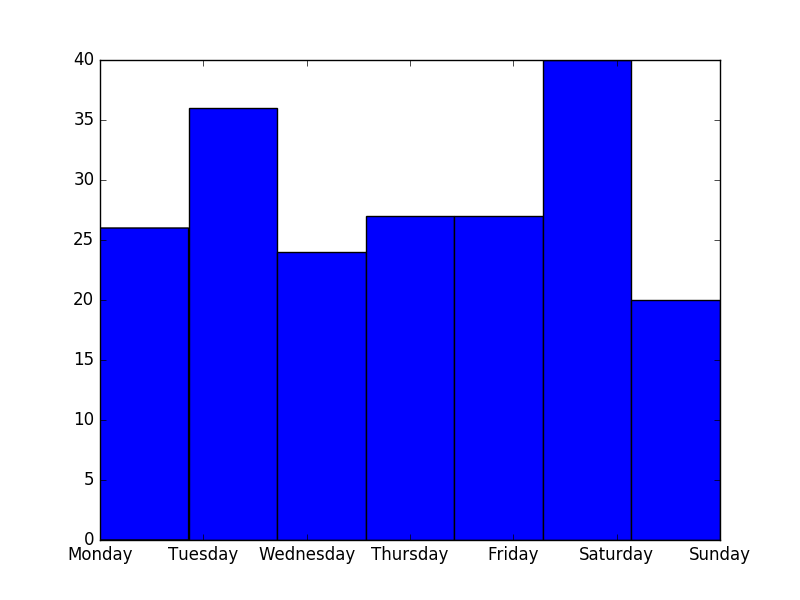
\includegraphics[width=4.16667in]{dow.png}

\subsubsection{\texorpdfstring{More \emph{DataFrame} Manipulation and
Plotting}{More DataFrame Manipulation and Plotting}}\label{more-dataframe-manipulation-and-plotting}

\texttt{DataFrame}s and \texttt{numpy} give us other ways to manipulate
data. For example, we can plot a histogram of the ages of violators like
this:

\begin{lstlisting}
>>> ages = data['Cited Person Age'].astype(int)
>>> fig = plt.figure()
>>> ax = fig.add_subplot(1, 1, 1)
>>> plt.hist(ages, bins=np.max(ages) - np.min(ages))
>>> plt.show()
\end{lstlisting}

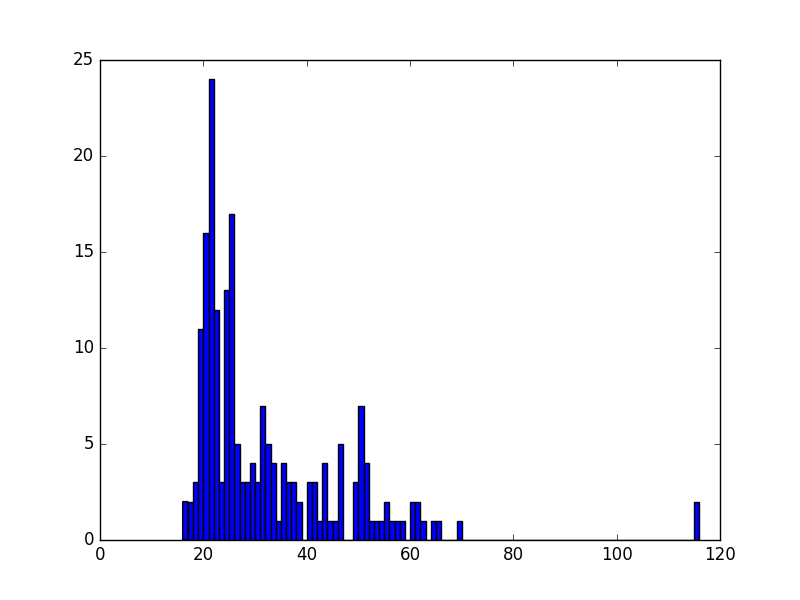
\includegraphics[width=4.16667in]{ages.png}

Surprisingly, we see some 116 year-old violators! This is probably an
error in the data, so we can remove these data points easily and plot
the histogram again:

\begin{lstlisting}
>>> ages = ages[ages < 100]
>>> fig = plt.figure()
>>> ax = fig.add_subplot(1, 1, 1)
>>> plt.hist(ages, bins=np.max(ages) - np.min(ages))
>>> plt.show()
\end{lstlisting}

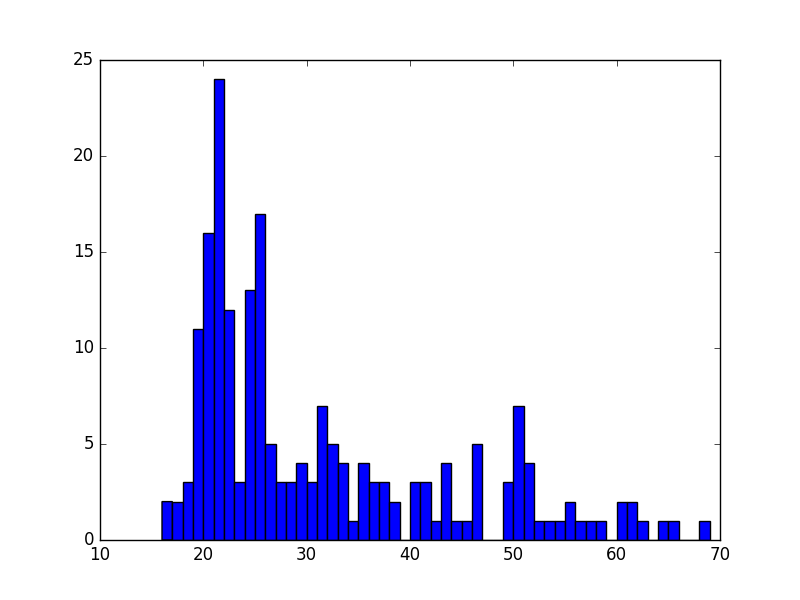
\includegraphics[width=4.16667in]{ages-filtered.png}

\subsubsection{Saving Plots to PDF}\label{saving-plots-to-pdf}

Oftentimes, you will want to save your \texttt{matplotlib} graph as a
PDF or an SVG file instead of just viewing it on your screen. For both,
we need to create a \texttt{figure} and plot the histogram as before:

\begin{lstlisting}
>>> fig = plt.figure()
>>> ax = fig.add_subplot(1, 1, 1)
>>> plt.hist(ages, bins=np.max(ages) - np.min(ages))
\end{lstlisting}

Then, instead of calling \texttt{plt.show()} we can invoke
\texttt{plt.savefig()} to save as SVG:

\begin{lstlisting}
>>> plt.savefig('hist.svg')
\end{lstlisting}

If we want to save the figure as PDF instead, we need to use the
\texttt{PdfPages} module together with \texttt{savefig()}:

\begin{lstlisting}
>>> import matplotlib.patches as mpatches
>>> from matplotlib.backends.backend_pdf import PdfPages   
>>> pp = PdfPages('hist.pdf')
>>> fig.savefig(pp, format='pdf')
>>> pp.close()
\end{lstlisting}

\subsubsection{Next Steps and Exercises}\label{next-steps-and-exercises}

There is a lot more to working with \texttt{pandas}, \texttt{numpy} and
\texttt{matplotlib} than we can show you here, but hopefully this
example has piqued your curiosity.

Don't worry if you don't understand everything in this example. For a
more detailed explanation on these modules and the examples we did,
please take a look at the tutorials below. The \texttt{numpy} and
\texttt{pandas} tutorials are mandatory if you want to be able to use
these modules, and the \texttt{matplotlib} gallery has many useful code
examples.

\subsection{Summary of Useful
Libraries}\label{summary-of-useful-libraries}

\subsubsection{Numpy}\label{numpy}

  \URL{http://www.numpy.org/}


According to the Numpy Web page "NumPy is a package for scientific
computing with Python. It contains a powerful N-dimensional array
object, sophisticated (broadcasting) functions, tools for integrating
C/C++ and Fortran code, useful linear algebra, Fourier transform, and
random number capabilities

Tutorial:
\url{https://docs.scipy.org/doc/numpy-dev/user/quickstart.html}

\subsubsection{MatplotLib}\label{matplotlib}

  \URL{http://matplotlib.org/}

According the the Matplotlib Web page, ``matplotlib is a python 2D
plotting library which produces publication quality figures in a variety
of hardcopy formats and interactive environments across platforms.
matplotlib can be used in python scripts, the python and ipython shell
(ala MATLAB®* or Mathematica®†), web application servers, and six
graphical user interface toolkits.''

Matplotlib Gallery: \url{http://matplotlib.org/gallery.html}

\subsubsection{Pandas}\label{pandas}

  \URL{http://pandas.pydata.org/}

According to the Pandas Web page, ``Pandas is a library library
providing high-performance, easy-to-use data structures and data
analysis tools for the Python programming language.''

In addition to access to charts via matplotlib it has elementary
functionality for conduction data analysis. Pandas may be very suitable
for your projects.

Tutorial: \url{http://pandas.pydata.org/pandas-docs/stable/10min.html}

Pandas Cheat Sheet:
\url{https://github.com/pandas-dev/pandas/blob/master/doc/cheatsheet/Pandas_Cheat_Sheet.pdf}

\subsection{Big Data Libraries}\label{other-useful-libraries}

\subsubsection{Scipy}\label{scipy}

  \URL{https://www.scipy.org/}

According to the SciPy Web page, ``SciPy (pronounced ``Sigh Pie'') is a
Python-based ecosystem of open-source software for mathematics, science,
and engineering. In particular, these are some of the core packages:

\begin{itemize}
\item NumPy
\item IPython
\item Pandas
\item Matplotlib
\item Sympy
\item SciPy library
\end{itemize}

It is thus an agglomeration of useful pacakes and will prbably sufice
for your projects in case you use Python.

\subsubsection{ggplot}\label{ggplot}

  \URL{http://ggplot.yhathq.com/}


According to the ggplot python Web page ggplot is a plotting system for
Python based on R's ggplot2. It allows to quickly generate some plots
quickly with little effort. Often it may be easier to use than
matplotlib directly.

\subsubsection{seaborn}\label{seaborn}

\URL{http://www.data-analysis-in-python.org/t_seaborn.html}

The good library for plotting is called seaborn which is build on top of
matplotlib. It provides high level templates for common statistical
plots.

\begin{itemize}
\item
  Gallery:
  \url{http://stanford.edu/~mwaskom/software/seaborn/examples/index.html}
\item
  Original Tutorial:
  \url{http://stanford.edu/~mwaskom/software/seaborn/tutorial.html}
\item
  Additional Tutorial:
  \url{https://stanford.edu/~mwaskom/software/seaborn/tutorial/distributions.html}
\end{itemize}

Here are some examples from a previous class:

\URL{https://github.com/bigdata-i523/hid231/blob/master/experiment/seaborn/seaborn-exercises.ipynb}
\URL{https://github.com/bigdata-i523/hid231/blob/master/experiment/learning-jupyter/learning_jupyter_notebook.ipynb}

\begin{exercise}\label{E:ipynb-export}
Take these examples and cretae sections in latex that can be added to
the book. Describe the process. 

1. export the ipynb as rst
2. use pandoc to export it to tex
3. do some cleanup on the tex files

Can this be automated with a cmd5 script such as
\begin{lstlisting}{bash}
cms ipynb [url=URL | file=FILE] --output FILENAME
\end{lstlisting}
\end{exercise}

\subsubsection{Bokeh}\label{bokeh}

Bokeh is an interactive visualization library with focus on web browsers
for display. Its goal is to provide a similar experience as D3.js

\begin{itemize}
\item
  URL: \url{http://bokeh.pydata.org/}
\item
  Gallery: \url{http://bokeh.pydata.org/en/latest/docs/gallery.html}
\end{itemize}

\subsubsection{pygal}\label{pygal}

Pygal is a simple API to produce graphs that can be easily embedded into
your Web pages. It contains annotations when you hover over data points.
It also allows to present the data in a table.

\URL{http://pygal.org/}


\subsubsection{Network and Graphs}\label{network-and-graphs}

\begin{itemize}
\tightlist
\item
  igraph: \url{http://www.pythonforsocialscientists.org/t_igraph.html}
\item
  networkx: \url{https://networkx.github.io/}
\end{itemize}

\subsubsection{REST}\label{rest}

\begin{itemize}
\tightlist
\item
  django REST FRamework \url{http://www.django-rest-framework.org/}
\item
  flask
  \url{https://blog.miguelgrinberg.com/post/designing-a-restful-api-with-python-and-flask}
\item
  requests
  \url{https://realpython.com/blog/python/api-integration-in-python/}
\item
  urllib2
  \url{http://rest.elkstein.org/2008/02/using-rest-in-python.html} (not
  recommended)
\item
  web
  \url{http://www.dreamsyssoft.com/python-scripting-tutorial/create-simple-rest-web-service-with-python.php}
  (not recommended)
\item
  bottle \url{http://bottlepy.org/docs/dev/index.html}
\item
  falcon \url{https://falconframework.org/}
\item
  eve \url{http://python-eve.org/}
\item
  \url{https://code.tutsplus.com/tutorials/building-rest-apis-using-eve--cms-22961}
\end{itemize}

\section{Parsing Data}

Being able to parse data is an important activity in the data analysis
process. Not all data may be following aspecific format and the data
may need to be extracted.


\subsection{notebook.md Parser}

We are using a notebook.md to communicate what students have done
throughout the semester. We like to make a simble cmd5 command that
parses the notebook.md file and check it upon correctness.

An example for a notebook.md file is lokated here 

\URL{https://raw.githubusercontent.com/bigdata-i523/sample-hid000/master/notebook.md}

The following code may inspire you

\URL{https://github.com/bigdata-i523/hid203/tree/master/experiment}

We like to implement the follwoing functionality and use docopts to
document the command.

\begin{lstlisting}
cms class notebook [--git=GITREPONAME] --verify hid

    verifies the correctness of the notebook.md file

cms class notebook [--git=GITREPONAME] --log

    displays the log of the notebook.md

cms class notebook [--git=GITREPONAME] --history

    displays a true or false for each week since the first occurance
    of the notebook.md file in the git repository
\end{lstlisting}

\begin{exercise}
  \label{E:notebook-md.1}
  Write a notebook.md parser
\end{exercise}

\begin{exercise}
  \label{E:notebook-md.2}
  How can this command be generalized to provide not only information
  for a student but to provide information for the class. Example: can
  we identify prefered days of when the notebooks are checked in. Can
  we identify a list of students that have not updated the notebok for
  a week?  Can we identify the list of student s that have updated the
  notebook for a week? 
\end{exercise}


\subsection{Video Length}

The Latex source of this class contains a macro to include videos.


Given a LateX file, can you create a table that includes the names of
all videos in that file and sums up the total viewing time. Previously
the document was stored in RST and the code from a previous student
may inspire you. Can you reqrite it in for LaTeX? 

\URL{https://github.com/bigdata-i523/hid107/blob/master/cloudmesh/bar/command/mycommand.py}


\begin{lstlisting}
cms class video list FILENAME --output=[tabular|longtable|csv|txt]

    prints the videolist in the given format. txt means it is just ASCII
\end{lstlisting}

\begin{comment}
The previous work even summarized the video length by chapter.

see: https://piazza.com/class/j5wll7vzylg25j?cid=325
\end{comment}

\begin{exercise}
Write a tool that extracts the information for video length. 
\end{exercise}

\begin{exercise}
Write a tool that finds all youtube urls that are not in a video latex
macro.
\end{exercise}

\subsection{Dask}
\index{Dask}

Many times operations need to be done on data in parallel to utilize
modern processor architectures.


Dask provides a {\em dynamic task scheduling} which is optimized for
computation. It is similar to other frameworks such as Airflow, Luigi,
Celery, or Make. HOwever it is specializing in optimized interactive
computational workloads.

Furthermore, Dask targets Big Data {\em collections} such as parallel
arrays, dataframes, and lists. Thes ecollections ar commonly found in
NumPy, Pandas, or Python iterators to larger-than-memory or
distributed environments. While using the Dask implementation we can
replace the original imports from the appropriate framework, replace
them with Dask imports and implicity use parallel collections that
utilize internally the dynamic task schedulers.

More information can be found at:

\URL{https://dask.pydata.org}

\begin{exercise}
Conduct a preformance study that showcases the difference of doing
parallel calculations in Dask, claculations in a framework such as
SciPy, and regular unthreaded python code.
\end{exercise}

